\documentclass[letter]{article}

\usepackage[english]{babel}
\usepackage[utf8x]{inputenc}
\usepackage[T1]{fontenc}
\usepackage[letterpaper, top=2cm,bottom=2cm,left=2cm,right=2cm,marginparwidth=1.75cm]{geometry}
\usepackage{amsmath}
\usepackage{graphicx}
\usepackage[colorinlistoftodos]{todonotes}
\usepackage[colorlinks=true, allcolors=blue]{hyperref}
\usepackage[numbered,framed]{matlab-prettifier}
\lstset{
	basicstyle=\small,
	breaklines=true
}

\title{Learning-Rate Decay for Generator}
\author{Mitch Hill, Erik Nijkamp}

\begin{document}
\maketitle

\begin{abstract}
The training of CoopNet on $32\times32$ image patches is non-trivial. The descriptor net appears to synthesize realistic and sharp images easily. The training seems relatively insensitive to varying learning parameters. In contrast, synthesis of sharp images by the generator net is hard. The training is very sensitive to variations in the parameters. We aim to identify relations between learning-rate and 'sharpness' from which we may formulate decay regimes.
\end{abstract}

\subsubsection*{Result}

\begin{table}[h!]
\centering
\begin{tabular}{cccc}
	exp & approach & gamma2 & loss\\
	\\[-1em]
	\hline 
	\\[-1em]
	(1) & step-wise decay & $(0.00035:100,\,0.000035:200,\,0.0000035:100)$ & unknown\\
	\\[-1em]
	(2) & step-wise decay $\times10$ & $(0.0005:100,\,0.0001:100,\,0.00005:100,\,0.00001:100,\,0.000005:100)\cdot10$ & $0.050311$\\
	\\[-1em]
	(3) & step-wise decay $\times2$ & $(0.0005:100,\,0.0001:100,\,0.00005:100,\,0.00001:100,\,0.000005:100)\cdot2.0$ & $0.066391$\\
	\\[-1em]
	(4) & step-wise decay $\times1$ & $(0.0005:100,\,0.0001:100,\,0.00005:100,\,0.00001:100,\,0.000005:100)\cdot1.0$ & $0.073952$\\
	\\[-1em]
	(5) & step-wise decay $\times.5$ & $(0.0005:100,\,0.0001:100,\,0.00005:100,\,0.00001:100,\,0.000005:100)\cdot0.5$ & $0.085113$\\
	\\[-1em]
	(6) & step-wise decay $\times.1$ & $(0.0005:100,\,0.0001:100,\,0.00005:100,\,0.00001:100,\,0.000005:100)\cdot0.1$ & $0.11982$\\
	\\[-1em]
	(7) & (2) increased & $(0.0003:100,\,0.0001:100,\,0.00005:100,\,0.00005:100,\,0.00001:100)\cdot10$ & $0.044032$\\
	\\[-1em]
	(8) & step-wise decay $\times20$ & $(0.0005:100,\,0.0001:100,\,0.00005:100,\,0.00001:100,\,0.000005:100)\cdot20$ & $0.053683$\\
	\\[-1em]
	(9) & log-space decay & $0.0005\cdot logspace(-2,-3,500)\cdot100$ & $0.059591$\\
	\\[-1em]
	(10) & log-space increased & $0.001\cdot logspace(-2,-3,500)\cdot100$ & $0.052407$\\
	\\[-1em]
	(11) & log-space long-tail & $0.001\cdot logspace(-2,-4,500)\cdot100$ & $0.064684$\\
	\\[-1em]
	(12) & lin-space decay & $0.0005\cdot linspace(1,0.01,500)$ & $0.054532$\\
\end{tabular}
\caption{Experiments and preliminary results.}
\end{table}

\newpage

\subsubsection*{Parameters}

\begin{lstlisting}
config.nIteration = 500;      
config.batchSize = 32;
                                
% sampling parameters
config.num_syn = 32;

% descriptor net1 parameters
config.Delta = 0.3;
config.Gamma = [0.0005*ones(1,100), 0.00005*ones(1,100), 0.00001*ones(1,100), 0.000005*ones(1,100), 0.000001*ones(1,100)];
config.refsig = 1;                                            
config.T = 40;             
                                                                                                   
% generator net2 parameters
config.Delta2 = 0.3;
config.refsig2 = 1;
config.s = 0.3;
config.real_ref = 1;
config.cap2 = 8;

% how many layers to learn
config.layer_to_learn = 1;

% image size
config.im_size = 32;
\end{lstlisting}

\newpage

\subsubsection*{Image patches from original texture}

\begin{table}[h!]
	\centering
	\begin{tabular}{cccc}
		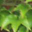
\includegraphics[width=0.17\textwidth]{../data/ivy2/512/1} &
		
\includegraphics[width=0.17\textwidth]{../data/ivy2/512/2} &
		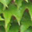
\includegraphics[width=0.17\textwidth]{../data/ivy2/512/3} &
		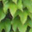
\includegraphics[width=0.17\textwidth]{../data/ivy2/512/4} \tabularnewline
		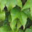
\includegraphics[width=0.17\textwidth]{../data/ivy2/512/5} &
		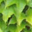
\includegraphics[width=0.17\textwidth]{../data/ivy2/512/6} &
		
\includegraphics[width=0.17\textwidth]{../data/ivy2/512/7} &
		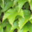
\includegraphics[width=0.17\textwidth]{../data/ivy2/512/8} \tabularnewline
		
\includegraphics[width=0.17\textwidth]{../data/ivy2/512/9} &
		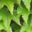
\includegraphics[width=0.17\textwidth]{../data/ivy2/512/10} &
		
\includegraphics[width=0.17\textwidth]{../data/ivy2/512/11} &
		
\includegraphics[width=0.17\textwidth]{../data/ivy2/512/12} \tabularnewline
		
\includegraphics[width=0.17\textwidth]{../data/ivy2/512/13} &
		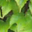
\includegraphics[width=0.17\textwidth]{../data/ivy2/512/14} &
		
\includegraphics[width=0.17\textwidth]{../data/ivy2/512/15} &
		
\includegraphics[width=0.17\textwidth]{../data/ivy2/512/16} \tabularnewline
		
\includegraphics[width=0.17\textwidth]{../data/ivy2/512/17} &
		
\includegraphics[width=0.17\textwidth]{../data/ivy2/512/18} &
		
\includegraphics[width=0.17\textwidth]{../data/ivy2/512/19} &
		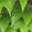
\includegraphics[width=0.17\textwidth]{../data/ivy2/512/20} \tabularnewline
		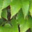
\includegraphics[width=0.17\textwidth]{../data/ivy2/512/21} &
		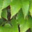
\includegraphics[width=0.17\textwidth]{../data/ivy2/512/21} &
		
\includegraphics[width=0.17\textwidth]{../data/ivy2/512/22} &
		
\includegraphics[width=0.17\textwidth]{../data/ivy2/512/23} \tabularnewline
	\end{tabular}
	\caption{Image patches sampled from original texture.}
\end{table}

\newpage

\subsubsection*{(1) exp\_texture\_512: step-wise decay - initial}

\begin{lstlisting}
config.Gamma2 = [0.00035*ones(1,100), 0.000035*ones(1,200), 0.0000035*ones(1,100)];
\end{lstlisting}

\begin{figure}[h!]
\centering
\includegraphics[width=0.7\textwidth]{../plots/ivy2/512_1/gamma2.png}
\caption{\label{fig:gamma1}Gamma2.}
\end{figure}

\begin{figure}[h!]
	\centering
	\includegraphics[width=0.7\textwidth]{../plots/ivy2/512_1/loss.png}
	\caption{\label{fig:gamma1}Loss (missing).}
\end{figure}

\newpage

\begin{table}[h!]
	\centering
	\begin{tabular}{c}
		ori\tabularnewline
		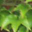
\includegraphics[width=0.17\textwidth]{../data/ivy2/512/1} \tabularnewline		
\includegraphics[width=0.17\textwidth]{../data/ivy2/512/2} \tabularnewline		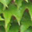
\includegraphics[width=0.17\textwidth]{../data/ivy2/512/3} \tabularnewline		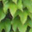
\includegraphics[width=0.17\textwidth]{../data/ivy2/512/4} \tabularnewline		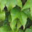
\includegraphics[width=0.17\textwidth]{../data/ivy2/512/5} \tabularnewline		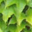
\includegraphics[width=0.17\textwidth]{../data/ivy2/512/6} \tabularnewline
	\end{tabular}
	\begin{tabular}{cc}
		syn & gen\tabularnewline
		
\includegraphics[width=0.17\textwidth]{../output/ims_syn/ivy2/512_1/syn_im1} & 
\includegraphics[width=0.17\textwidth]{../output/ims_gen/ivy2/512_1/gen_im1} \tabularnewline
		
\includegraphics[width=0.17\textwidth]{../output/ims_syn/ivy2/512_1/syn_im2} & 
\includegraphics[width=0.17\textwidth]{../output/ims_gen/ivy2/512_1/gen_im2} \tabularnewline
		
\includegraphics[width=0.17\textwidth]{../output/ims_syn/ivy2/512_1/syn_im3} & 
\includegraphics[width=0.17\textwidth]{../output/ims_gen/ivy2/512_1/gen_im3} \tabularnewline
		
\includegraphics[width=0.17\textwidth]{../output/ims_syn/ivy2/512_1/syn_im4} & 
\includegraphics[width=0.17\textwidth]{../output/ims_gen/ivy2/512_1/gen_im4} \tabularnewline
		
\includegraphics[width=0.17\textwidth]{../output/ims_syn/ivy2/512_1/syn_im5} & 
\includegraphics[width=0.17\textwidth]{../output/ims_gen/ivy2/512_1/gen_im5} \tabularnewline
		
\includegraphics[width=0.17\textwidth]{../output/ims_syn/ivy2/512_1/syn_im6} & 
\includegraphics[width=0.17\textwidth]{../output/ims_gen/ivy2/512_1/gen_im6} \tabularnewline
	\end{tabular}
	\begin{tabular}{cc}
		syn & gen\tabularnewline
		
\includegraphics[width=0.17\textwidth]{../output/ims_syn/ivy2/512_1/syn_im7} & 
\includegraphics[width=0.17\textwidth]{../output/ims_gen/ivy2/512_1/gen_im7} \tabularnewline
		
\includegraphics[width=0.17\textwidth]{../output/ims_syn/ivy2/512_1/syn_im8} & 
\includegraphics[width=0.17\textwidth]{../output/ims_gen/ivy2/512_1/gen_im8} \tabularnewline
		
\includegraphics[width=0.17\textwidth]{../output/ims_syn/ivy2/512_1/syn_im9} & 
\includegraphics[width=0.17\textwidth]{../output/ims_gen/ivy2/512_1/gen_im9} \tabularnewline
		\includegraphics[width=0.17\textwidth]{../output/ims_syn/ivy2/512_1/syn_im10} & \includegraphics[width=0.17\textwidth]{../output/ims_gen/ivy2/512_1/gen_im10} \tabularnewline
		\includegraphics[width=0.17\textwidth]{../output/ims_syn/ivy2/512_1/syn_im11} & \includegraphics[width=0.17\textwidth]{../output/ims_gen/ivy2/512_1/gen_im11} \tabularnewline
		\includegraphics[width=0.17\textwidth]{../output/ims_syn/ivy2/512_1/syn_im12} & \includegraphics[width=0.17\textwidth]{../output/ims_gen/ivy2/512_1/gen_im12} \tabularnewline
	\end{tabular}
	\caption{Descriptor and generator images}
\end{table}

\newpage

\subsubsection*{(2) exp\_texture\_512\_2: step-wise decay - $\times10.0$}

\begin{lstlisting}
config.Gamma2 = [0.0005*ones(1,100), 0.0001*ones(1,100), 0.00005*ones(1,100), 0.00001*ones(1,100), 0.000005*ones(1,100)] * 10;
\end{lstlisting}

\begin{figure}[h!]
	\centering
	\includegraphics[width=0.7\textwidth]{../plots/ivy2/512_2/gamma2.png}
	\caption{\label{fig:gamma1}Gamma2.}
\end{figure}

\begin{figure}[h!]
	\centering
	\includegraphics[width=0.7\textwidth]{../plots/ivy2/512_2/loss.png}
	\caption{\label{fig:gamma1}Loss.}
\end{figure}

\newpage

\begin{table}[h!]
	\centering
	\begin{tabular}{c}
		ori\tabularnewline
		\includegraphics[width=0.17\textwidth]{../data/ivy2/512/1} \tabularnewline		\includegraphics[width=0.17\textwidth]{../data/ivy2/512/2} \tabularnewline		\includegraphics[width=0.17\textwidth]{../data/ivy2/512/3} \tabularnewline		\includegraphics[width=0.17\textwidth]{../data/ivy2/512/4} \tabularnewline		\includegraphics[width=0.17\textwidth]{../data/ivy2/512/5} \tabularnewline		\includegraphics[width=0.17\textwidth]{../data/ivy2/512/6} \tabularnewline
	\end{tabular}
	\begin{tabular}{cc}
		syn & gen\tabularnewline
		\includegraphics[width=0.17\textwidth]{../output/ims_syn/ivy2/512_2/syn_im1} & \includegraphics[width=0.17\textwidth]{../output/ims_gen/ivy2/512_2/gen_im1} \tabularnewline
		\includegraphics[width=0.17\textwidth]{../output/ims_syn/ivy2/512_2/syn_im2} & \includegraphics[width=0.17\textwidth]{../output/ims_gen/ivy2/512_2/gen_im2} \tabularnewline
		\includegraphics[width=0.17\textwidth]{../output/ims_syn/ivy2/512_2/syn_im3} & \includegraphics[width=0.17\textwidth]{../output/ims_gen/ivy2/512_2/gen_im3} \tabularnewline
		\includegraphics[width=0.17\textwidth]{../output/ims_syn/ivy2/512_2/syn_im4} & \includegraphics[width=0.17\textwidth]{../output/ims_gen/ivy2/512_2/gen_im4} \tabularnewline
		\includegraphics[width=0.17\textwidth]{../output/ims_syn/ivy2/512_2/syn_im15} & \includegraphics[width=0.17\textwidth]{../output/ims_gen/ivy2/512_2/gen_im15} \tabularnewline
		\includegraphics[width=0.17\textwidth]{../output/ims_syn/ivy2/512_2/syn_im6} & \includegraphics[width=0.17\textwidth]{../output/ims_gen/ivy2/512_2/gen_im6} \tabularnewline
	\end{tabular}
	\begin{tabular}{cc}
		syn & gen\tabularnewline
		\includegraphics[width=0.17\textwidth]{../output/ims_syn/ivy2/512_2/syn_im7} & \includegraphics[width=0.17\textwidth]{../output/ims_gen/ivy2/512_2/gen_im7} \tabularnewline
		\includegraphics[width=0.17\textwidth]{../output/ims_syn/ivy2/512_2/syn_im8} & \includegraphics[width=0.17\textwidth]{../output/ims_gen/ivy2/512_2/gen_im8} \tabularnewline
		\includegraphics[width=0.17\textwidth]{../output/ims_syn/ivy2/512_2/syn_im9} & \includegraphics[width=0.17\textwidth]{../output/ims_gen/ivy2/512_2/gen_im9} \tabularnewline
		\includegraphics[width=0.17\textwidth]{../output/ims_syn/ivy2/512_2/syn_im10} & \includegraphics[width=0.17\textwidth]{../output/ims_gen/ivy2/512_2/gen_im10} \tabularnewline
		\includegraphics[width=0.17\textwidth]{../output/ims_syn/ivy2/512_2/syn_im11} & \includegraphics[width=0.17\textwidth]{../output/ims_gen/ivy2/512_2/gen_im11} \tabularnewline
		\includegraphics[width=0.17\textwidth]{../output/ims_syn/ivy2/512_2/syn_im12} & \includegraphics[width=0.17\textwidth]{../output/ims_gen/ivy2/512_2/gen_im12} \tabularnewline
	\end{tabular}
	\caption{Descriptor and generator images}
\end{table}

\newpage

\subsubsection*{(3) exp\_texture\_512\_3: step-wise decay - $\times2.0$}

\begin{lstlisting}
config.Gamma2 = [0.0005*ones(1,100), 0.0001*ones(1,100), 0.00005*ones(1,100), 0.00001*ones(1,100), 0.000005*ones(1,100)] * 2;
\end{lstlisting}

\begin{figure}[h!]
	\centering
	\includegraphics[width=0.7\textwidth]{../plots/ivy2/512_3/gamma2.png}
	\caption{\label{fig:gamma1}Gamma2.}
\end{figure}

\begin{figure}[h!]
	\centering
	\includegraphics[width=0.7\textwidth]{../plots/ivy2/512_3/loss.png}
	\caption{\label{fig:gamma1}Loss.}
\end{figure}

\newpage

\begin{table}[h!]
	\centering
	\begin{tabular}{c}
		ori\tabularnewline
		\includegraphics[width=0.17\textwidth]{../data/ivy2/512/1} \tabularnewline		\includegraphics[width=0.17\textwidth]{../data/ivy2/512/2} \tabularnewline		\includegraphics[width=0.17\textwidth]{../data/ivy2/512/3} \tabularnewline		\includegraphics[width=0.17\textwidth]{../data/ivy2/512/4} \tabularnewline		\includegraphics[width=0.17\textwidth]{../data/ivy2/512/5} \tabularnewline		\includegraphics[width=0.17\textwidth]{../data/ivy2/512/6} \tabularnewline
	\end{tabular}
	\begin{tabular}{cc}
		syn & gen\tabularnewline
		\includegraphics[width=0.17\textwidth]{../output/ims_syn/ivy2/512_3/syn_im1} & \includegraphics[width=0.17\textwidth]{../output/ims_gen/ivy2/512_3/gen_im1} \tabularnewline
		\includegraphics[width=0.17\textwidth]{../output/ims_syn/ivy2/512_3/syn_im2} & \includegraphics[width=0.17\textwidth]{../output/ims_gen/ivy2/512_3/gen_im2} \tabularnewline
		\includegraphics[width=0.17\textwidth]{../output/ims_syn/ivy2/512_3/syn_im3} & \includegraphics[width=0.17\textwidth]{../output/ims_gen/ivy2/512_3/gen_im3} \tabularnewline
		\includegraphics[width=0.17\textwidth]{../output/ims_syn/ivy2/512_3/syn_im4} & \includegraphics[width=0.17\textwidth]{../output/ims_gen/ivy2/512_3/gen_im4} \tabularnewline
		\includegraphics[width=0.17\textwidth]{../output/ims_syn/ivy2/512_3/syn_im5} & \includegraphics[width=0.17\textwidth]{../output/ims_gen/ivy2/512_3/gen_im5} \tabularnewline
		\includegraphics[width=0.17\textwidth]{../output/ims_syn/ivy2/512_3/syn_im6} & \includegraphics[width=0.17\textwidth]{../output/ims_gen/ivy2/512_3/gen_im6} \tabularnewline
	\end{tabular}
	\begin{tabular}{cc}
		syn & gen\tabularnewline
		\includegraphics[width=0.17\textwidth]{../output/ims_syn/ivy2/512_3/syn_im7} & \includegraphics[width=0.17\textwidth]{../output/ims_gen/ivy2/512_3/gen_im7} \tabularnewline
		\includegraphics[width=0.17\textwidth]{../output/ims_syn/ivy2/512_3/syn_im8} & \includegraphics[width=0.17\textwidth]{../output/ims_gen/ivy2/512_3/gen_im8} \tabularnewline
		\includegraphics[width=0.17\textwidth]{../output/ims_syn/ivy2/512_3/syn_im9} & \includegraphics[width=0.17\textwidth]{../output/ims_gen/ivy2/512_3/gen_im9} \tabularnewline
		\includegraphics[width=0.17\textwidth]{../output/ims_syn/ivy2/512_3/syn_im10} & \includegraphics[width=0.17\textwidth]{../output/ims_gen/ivy2/512_3/gen_im10} \tabularnewline
		\includegraphics[width=0.17\textwidth]{../output/ims_syn/ivy2/512_3/syn_im11} & \includegraphics[width=0.17\textwidth]{../output/ims_gen/ivy2/512_3/gen_im11} \tabularnewline
		\includegraphics[width=0.17\textwidth]{../output/ims_syn/ivy2/512_3/syn_im12} & \includegraphics[width=0.17\textwidth]{../output/ims_gen/ivy2/512_3/gen_im12} \tabularnewline
	\end{tabular}
	\caption{Descriptor and generator images}
\end{table}

\newpage

\subsubsection*{(4) exp\_texture\_512\_4: step-wise - $\times1.0$}

\begin{lstlisting}
config.Gamma2 = [0.0005*ones(1,100), 0.0001*ones(1,100), 0.00005*ones(1,100), 0.00001*ones(1,100), 0.000005*ones(1,100)] * 1;
\end{lstlisting}

\begin{figure}[h!]
	\centering
	\includegraphics[width=0.7\textwidth]{../plots/ivy2/512_4/gamma2.png}
	\caption{\label{fig:gamma1}Gamma2.}
\end{figure}

\begin{figure}[h!]
	\centering
	\includegraphics[width=0.7\textwidth]{../plots/ivy2/512_4/loss.png}
	\caption{\label{fig:gamma1}Loss.}
\end{figure}

\newpage

\begin{table}[h!]
	\centering
	\begin{tabular}{c}
		ori\tabularnewline
		\includegraphics[width=0.17\textwidth]{../data/ivy2/512/1} \tabularnewline		\includegraphics[width=0.17\textwidth]{../data/ivy2/512/2} \tabularnewline		\includegraphics[width=0.17\textwidth]{../data/ivy2/512/3} \tabularnewline		\includegraphics[width=0.17\textwidth]{../data/ivy2/512/4} \tabularnewline		\includegraphics[width=0.17\textwidth]{../data/ivy2/512/5} \tabularnewline		\includegraphics[width=0.17\textwidth]{../data/ivy2/512/6} \tabularnewline
	\end{tabular}
	\begin{tabular}{cc}
		syn & gen\tabularnewline
		\includegraphics[width=0.17\textwidth]{../output/ims_syn/ivy2/512_4/syn_im1} & \includegraphics[width=0.17\textwidth]{../output/ims_gen/ivy2/512_4/gen_im1} \tabularnewline
		\includegraphics[width=0.17\textwidth]{../output/ims_syn/ivy2/512_4/syn_im2} & \includegraphics[width=0.17\textwidth]{../output/ims_gen/ivy2/512_4/gen_im2} \tabularnewline
		\includegraphics[width=0.17\textwidth]{../output/ims_syn/ivy2/512_4/syn_im3} & \includegraphics[width=0.17\textwidth]{../output/ims_gen/ivy2/512_4/gen_im3} \tabularnewline
		\includegraphics[width=0.17\textwidth]{../output/ims_syn/ivy2/512_4/syn_im4} & \includegraphics[width=0.17\textwidth]{../output/ims_gen/ivy2/512_4/gen_im4} \tabularnewline
		\includegraphics[width=0.17\textwidth]{../output/ims_syn/ivy2/512_4/syn_im5} & \includegraphics[width=0.17\textwidth]{../output/ims_gen/ivy2/512_4/gen_im5} \tabularnewline
		\includegraphics[width=0.17\textwidth]{../output/ims_syn/ivy2/512_4/syn_im6} & \includegraphics[width=0.17\textwidth]{../output/ims_gen/ivy2/512_4/gen_im6} \tabularnewline
	\end{tabular}
	\begin{tabular}{cc}
		syn & gen\tabularnewline
		\includegraphics[width=0.17\textwidth]{../output/ims_syn/ivy2/512_4/syn_im7} & \includegraphics[width=0.17\textwidth]{../output/ims_gen/ivy2/512_4/gen_im7} \tabularnewline
		\includegraphics[width=0.17\textwidth]{../output/ims_syn/ivy2/512_4/syn_im8} & \includegraphics[width=0.17\textwidth]{../output/ims_gen/ivy2/512_4/gen_im8} \tabularnewline
		\includegraphics[width=0.17\textwidth]{../output/ims_syn/ivy2/512_4/syn_im9} & \includegraphics[width=0.17\textwidth]{../output/ims_gen/ivy2/512_4/gen_im9} \tabularnewline
		\includegraphics[width=0.17\textwidth]{../output/ims_syn/ivy2/512_4/syn_im10} & \includegraphics[width=0.17\textwidth]{../output/ims_gen/ivy2/512_4/gen_im10} \tabularnewline
		\includegraphics[width=0.17\textwidth]{../output/ims_syn/ivy2/512_4/syn_im11} & \includegraphics[width=0.17\textwidth]{../output/ims_gen/ivy2/512_4/gen_im11} \tabularnewline
		\includegraphics[width=0.17\textwidth]{../output/ims_syn/ivy2/512_4/syn_im12} & \includegraphics[width=0.17\textwidth]{../output/ims_gen/ivy2/512_4/gen_im12} \tabularnewline
	\end{tabular}
	\caption{Descriptor and generator images}
\end{table}

\newpage

\subsubsection*{(5) exp\_texture\_512\_5: step-wise - $\times0.5$}

\begin{lstlisting}
config.Gamma2 = [0.0005*ones(1,100), 0.0001*ones(1,100), 0.00005*ones(1,100), 0.00001*ones(1,100), 0.000005*ones(1,100)] / 2;
\end{lstlisting}

\begin{figure}[h!]
	\centering
	\includegraphics[width=0.7\textwidth]{../plots/ivy2/512_5/gamma2.png}
	\caption{\label{fig:gamma1}Gamma2.}
\end{figure}

\begin{figure}[h!]
	\centering
	\includegraphics[width=0.7\textwidth]{../plots/ivy2/512_5/loss.png}
	\caption{\label{fig:gamma1}Loss.}
\end{figure}

\newpage

\begin{table}[h!]
	\centering
	\begin{tabular}{c}
		ori\tabularnewline
		\includegraphics[width=0.17\textwidth]{../data/ivy2/512/1} \tabularnewline		\includegraphics[width=0.17\textwidth]{../data/ivy2/512/2} \tabularnewline		\includegraphics[width=0.17\textwidth]{../data/ivy2/512/3} \tabularnewline		\includegraphics[width=0.17\textwidth]{../data/ivy2/512/4} \tabularnewline		\includegraphics[width=0.17\textwidth]{../data/ivy2/512/5} \tabularnewline		\includegraphics[width=0.17\textwidth]{../data/ivy2/512/6} \tabularnewline
	\end{tabular}
	\begin{tabular}{cc}
		syn & gen\tabularnewline
		\includegraphics[width=0.17\textwidth]{../output/ims_syn/ivy2/512_5/syn_im1} & \includegraphics[width=0.17\textwidth]{../output/ims_gen/ivy2/512_5/gen_im1} \tabularnewline
		\includegraphics[width=0.17\textwidth]{../output/ims_syn/ivy2/512_5/syn_im2} & \includegraphics[width=0.17\textwidth]{../output/ims_gen/ivy2/512_5/gen_im2} \tabularnewline
		\includegraphics[width=0.17\textwidth]{../output/ims_syn/ivy2/512_5/syn_im3} & \includegraphics[width=0.17\textwidth]{../output/ims_gen/ivy2/512_5/gen_im3} \tabularnewline
		\includegraphics[width=0.17\textwidth]{../output/ims_syn/ivy2/512_5/syn_im4} & \includegraphics[width=0.17\textwidth]{../output/ims_gen/ivy2/512_5/gen_im4} \tabularnewline
		\includegraphics[width=0.17\textwidth]{../output/ims_syn/ivy2/512_5/syn_im5} & \includegraphics[width=0.17\textwidth]{../output/ims_gen/ivy2/512_5/gen_im5} \tabularnewline
		\includegraphics[width=0.17\textwidth]{../output/ims_syn/ivy2/512_5/syn_im6} & \includegraphics[width=0.17\textwidth]{../output/ims_gen/ivy2/512_5/gen_im6} \tabularnewline
	\end{tabular}
	\begin{tabular}{cc}
		syn & gen\tabularnewline
		\includegraphics[width=0.17\textwidth]{../output/ims_syn/ivy2/512_5/syn_im7} & \includegraphics[width=0.17\textwidth]{../output/ims_gen/ivy2/512_5/gen_im7} \tabularnewline
		\includegraphics[width=0.17\textwidth]{../output/ims_syn/ivy2/512_5/syn_im8} & \includegraphics[width=0.17\textwidth]{../output/ims_gen/ivy2/512_5/gen_im8} \tabularnewline
		\includegraphics[width=0.17\textwidth]{../output/ims_syn/ivy2/512_5/syn_im9} & \includegraphics[width=0.17\textwidth]{../output/ims_gen/ivy2/512_5/gen_im9} \tabularnewline
		\includegraphics[width=0.17\textwidth]{../output/ims_syn/ivy2/512_5/syn_im10} & \includegraphics[width=0.17\textwidth]{../output/ims_gen/ivy2/512_5/gen_im10} \tabularnewline
		\includegraphics[width=0.17\textwidth]{../output/ims_syn/ivy2/512_5/syn_im11} & \includegraphics[width=0.17\textwidth]{../output/ims_gen/ivy2/512_5/gen_im11} \tabularnewline
		\includegraphics[width=0.17\textwidth]{../output/ims_syn/ivy2/512_5/syn_im12} & \includegraphics[width=0.17\textwidth]{../output/ims_gen/ivy2/512_5/gen_im12} \tabularnewline
	\end{tabular}
	\caption{Descriptor and generator images}
\end{table}
\newpage

\subsubsection*{(6) exp\_texture\_512\_6: step-wise - $\times0.1$}

\begin{lstlisting}
config.Gamma2 = [0.0005*ones(1,100), 0.0001*ones(1,100), 0.00005*ones(1,100), 0.00001*ones(1,100), 0.000005*ones(1,100)] / 10; % decreased 
\end{lstlisting}

\begin{figure}[h!]
	\centering
	\includegraphics[width=0.7\textwidth]{../plots/ivy2/512_6/gamma2.png}
	\caption{\label{fig:gamma1}Gamma2.}
\end{figure}

\begin{figure}[h!]
	\centering
	\includegraphics[width=0.7\textwidth]{../plots/ivy2/512_6/loss.png}
	\caption{\label{fig:gamma1}Loss.}
\end{figure}

\newpage

\begin{table}[h!]
	\centering
	\begin{tabular}{c}
		ori\tabularnewline
		\includegraphics[width=0.17\textwidth]{../data/ivy2/512/1} \tabularnewline		\includegraphics[width=0.17\textwidth]{../data/ivy2/512/2} \tabularnewline		\includegraphics[width=0.17\textwidth]{../data/ivy2/512/3} \tabularnewline		\includegraphics[width=0.17\textwidth]{../data/ivy2/512/4} \tabularnewline		\includegraphics[width=0.17\textwidth]{../data/ivy2/512/5} \tabularnewline		\includegraphics[width=0.17\textwidth]{../data/ivy2/512/6} \tabularnewline
	\end{tabular}
	\begin{tabular}{cc}
		syn & gen\tabularnewline
		\includegraphics[width=0.17\textwidth]{../output/ims_syn/ivy2/512_6/syn_im1} & \includegraphics[width=0.17\textwidth]{../output/ims_gen/ivy2/512_6/gen_im1} \tabularnewline
		\includegraphics[width=0.17\textwidth]{../output/ims_syn/ivy2/512_6/syn_im2} & \includegraphics[width=0.17\textwidth]{../output/ims_gen/ivy2/512_6/gen_im2} \tabularnewline
		\includegraphics[width=0.17\textwidth]{../output/ims_syn/ivy2/512_6/syn_im3} & \includegraphics[width=0.17\textwidth]{../output/ims_gen/ivy2/512_6/gen_im3} \tabularnewline
		\includegraphics[width=0.17\textwidth]{../output/ims_syn/ivy2/512_6/syn_im4} & \includegraphics[width=0.17\textwidth]{../output/ims_gen/ivy2/512_6/gen_im4} \tabularnewline
		\includegraphics[width=0.17\textwidth]{../output/ims_syn/ivy2/512_6/syn_im5} & \includegraphics[width=0.17\textwidth]{../output/ims_gen/ivy2/512_6/gen_im5} \tabularnewline
		\includegraphics[width=0.17\textwidth]{../output/ims_syn/ivy2/512_6/syn_im6} & \includegraphics[width=0.17\textwidth]{../output/ims_gen/ivy2/512_6/gen_im6} \tabularnewline
	\end{tabular}
	\begin{tabular}{cc}
		syn & gen\tabularnewline
		\includegraphics[width=0.17\textwidth]{../output/ims_syn/ivy2/512_6/syn_im7} & \includegraphics[width=0.17\textwidth]{../output/ims_gen/ivy2/512_6/gen_im7} \tabularnewline
		\includegraphics[width=0.17\textwidth]{../output/ims_syn/ivy2/512_6/syn_im8} & \includegraphics[width=0.17\textwidth]{../output/ims_gen/ivy2/512_6/gen_im8} \tabularnewline
		\includegraphics[width=0.17\textwidth]{../output/ims_syn/ivy2/512_6/syn_im9} & \includegraphics[width=0.17\textwidth]{../output/ims_gen/ivy2/512_6/gen_im9} \tabularnewline
		\includegraphics[width=0.17\textwidth]{../output/ims_syn/ivy2/512_6/syn_im10} & \includegraphics[width=0.17\textwidth]{../output/ims_gen/ivy2/512_6/gen_im10} \tabularnewline
		\includegraphics[width=0.17\textwidth]{../output/ims_syn/ivy2/512_6/syn_im11} & \includegraphics[width=0.17\textwidth]{../output/ims_gen/ivy2/512_6/gen_im11} \tabularnewline
		\includegraphics[width=0.17\textwidth]{../output/ims_syn/ivy2/512_6/syn_im12} & \includegraphics[width=0.17\textwidth]{../output/ims_gen/ivy2/512_6/gen_im12} \tabularnewline
	\end{tabular}
	\caption{Descriptor and generator images}
\end{table}
\newpage

\subsubsection*{(7) exp\_texture\_512\_7: step-wise - (2) increased middle}

\begin{lstlisting}
config.Gamma2 = [0.0003*ones(1,100), 0.0001*ones(1,100), 0.00005*ones(1,100), 0.00005*ones(1,100), 0.00001*ones(1,100)] * 10; % (2) lower gamma in beginning, higher in middle 

\end{lstlisting}

\begin{figure}[h!]
	\centering
	\includegraphics[width=0.7\textwidth]{../plots/ivy2/512_7/gamma2.png}
	\caption{\label{fig:gamma1}Gamma2.}
\end{figure}

\begin{figure}[h!]
	\centering
	\includegraphics[width=0.7\textwidth]{../plots/ivy2/512_7/loss.png}
	\caption{\label{fig:gamma1}Loss.}
\end{figure}

\newpage

\begin{table}[h!]
	\centering
	\begin{tabular}{c}
		ori\tabularnewline
		\includegraphics[width=0.17\textwidth]{../data/ivy2/512/1} \tabularnewline		\includegraphics[width=0.17\textwidth]{../data/ivy2/512/2} \tabularnewline		\includegraphics[width=0.17\textwidth]{../data/ivy2/512/3} \tabularnewline		\includegraphics[width=0.17\textwidth]{../data/ivy2/512/4} \tabularnewline		\includegraphics[width=0.17\textwidth]{../data/ivy2/512/5} \tabularnewline		\includegraphics[width=0.17\textwidth]{../data/ivy2/512/6} \tabularnewline
	\end{tabular}
	\begin{tabular}{cc}
		syn & gen\tabularnewline
		\includegraphics[width=0.17\textwidth]{../output/ims_syn/ivy2/512_7/syn_im1} & \includegraphics[width=0.17\textwidth]{../output/ims_gen/ivy2/512_7/gen_im1} \tabularnewline
		\includegraphics[width=0.17\textwidth]{../output/ims_syn/ivy2/512_7/syn_im2} & \includegraphics[width=0.17\textwidth]{../output/ims_gen/ivy2/512_7/gen_im2} \tabularnewline
		\includegraphics[width=0.17\textwidth]{../output/ims_syn/ivy2/512_7/syn_im3} & \includegraphics[width=0.17\textwidth]{../output/ims_gen/ivy2/512_7/gen_im3} \tabularnewline
		\includegraphics[width=0.17\textwidth]{../output/ims_syn/ivy2/512_7/syn_im4} & \includegraphics[width=0.17\textwidth]{../output/ims_gen/ivy2/512_7/gen_im4} \tabularnewline
		\includegraphics[width=0.17\textwidth]{../output/ims_syn/ivy2/512_7/syn_im5} & \includegraphics[width=0.17\textwidth]{../output/ims_gen/ivy2/512_7/gen_im5} \tabularnewline
		\includegraphics[width=0.17\textwidth]{../output/ims_syn/ivy2/512_7/syn_im6} & \includegraphics[width=0.17\textwidth]{../output/ims_gen/ivy2/512_7/gen_im6} \tabularnewline
	\end{tabular}
	\begin{tabular}{cc}
		syn & gen\tabularnewline
		\includegraphics[width=0.17\textwidth]{../output/ims_syn/ivy2/512_7/syn_im7} & \includegraphics[width=0.17\textwidth]{../output/ims_gen/ivy2/512_7/gen_im7} \tabularnewline
		\includegraphics[width=0.17\textwidth]{../output/ims_syn/ivy2/512_7/syn_im8} & \includegraphics[width=0.17\textwidth]{../output/ims_gen/ivy2/512_7/gen_im8} \tabularnewline
		\includegraphics[width=0.17\textwidth]{../output/ims_syn/ivy2/512_7/syn_im9} & \includegraphics[width=0.17\textwidth]{../output/ims_gen/ivy2/512_7/gen_im9} \tabularnewline
		\includegraphics[width=0.17\textwidth]{../output/ims_syn/ivy2/512_7/syn_im10} & \includegraphics[width=0.17\textwidth]{../output/ims_gen/ivy2/512_7/gen_im10} \tabularnewline
		\includegraphics[width=0.17\textwidth]{../output/ims_syn/ivy2/512_7/syn_im11} & \includegraphics[width=0.17\textwidth]{../output/ims_gen/ivy2/512_7/gen_im11} \tabularnewline
		\includegraphics[width=0.17\textwidth]{../output/ims_syn/ivy2/512_7/syn_im12} & \includegraphics[width=0.17\textwidth]{../output/ims_gen/ivy2/512_7/gen_im12} \tabularnewline
	\end{tabular}
	\caption{Descriptor and generator images}
\end{table}
\newpage

\subsubsection*{(8) exp\_texture\_512\_8: step-wise - $\times20$}

\begin{lstlisting}
config.Gamma2 = [0.0005*ones(1,100), 0.0001*ones(1,100), 0.00005*ones(1,100), 0.00001*ones(1,100), 0.000005*ones(1,100)] * 20; % increased 
\end{lstlisting}

\begin{figure}[h!]
	\centering
	\includegraphics[width=0.7\textwidth]{../plots/ivy2/512_8/gamma2.png}
	\caption{\label{fig:gamma1}Gamma2.}
\end{figure}

\begin{figure}[h!]
	\centering
	\includegraphics[width=0.7\textwidth]{../plots/ivy2/512_8/loss.png}
	\caption{\label{fig:gamma1}Loss.}
\end{figure}

\newpage

\begin{table}[h!]
	\centering
	\begin{tabular}{c}
		ori\tabularnewline
		\includegraphics[width=0.17\textwidth]{../data/ivy2/512/1} \tabularnewline		\includegraphics[width=0.17\textwidth]{../data/ivy2/512/2} \tabularnewline		\includegraphics[width=0.17\textwidth]{../data/ivy2/512/3} \tabularnewline		\includegraphics[width=0.17\textwidth]{../data/ivy2/512/4} \tabularnewline		\includegraphics[width=0.17\textwidth]{../data/ivy2/512/5} \tabularnewline		\includegraphics[width=0.17\textwidth]{../data/ivy2/512/6} \tabularnewline
	\end{tabular}
	\begin{tabular}{cc}
		syn & gen\tabularnewline
		\includegraphics[width=0.17\textwidth]{../output/ims_syn/ivy2/512_8/syn_im1} & \includegraphics[width=0.17\textwidth]{../output/ims_gen/ivy2/512_8/gen_im1} \tabularnewline
		\includegraphics[width=0.17\textwidth]{../output/ims_syn/ivy2/512_8/syn_im2} & \includegraphics[width=0.17\textwidth]{../output/ims_gen/ivy2/512_8/gen_im2} \tabularnewline
		\includegraphics[width=0.17\textwidth]{../output/ims_syn/ivy2/512_8/syn_im3} & \includegraphics[width=0.17\textwidth]{../output/ims_gen/ivy2/512_8/gen_im3} \tabularnewline
		\includegraphics[width=0.17\textwidth]{../output/ims_syn/ivy2/512_8/syn_im4} & \includegraphics[width=0.17\textwidth]{../output/ims_gen/ivy2/512_8/gen_im4} \tabularnewline
		\includegraphics[width=0.17\textwidth]{../output/ims_syn/ivy2/512_8/syn_im5} & \includegraphics[width=0.17\textwidth]{../output/ims_gen/ivy2/512_8/gen_im5} \tabularnewline
		\includegraphics[width=0.17\textwidth]{../output/ims_syn/ivy2/512_8/syn_im6} & \includegraphics[width=0.17\textwidth]{../output/ims_gen/ivy2/512_8/gen_im6} \tabularnewline
	\end{tabular}
	\begin{tabular}{cc}
		syn & gen\tabularnewline
		\includegraphics[width=0.17\textwidth]{../output/ims_syn/ivy2/512_8/syn_im7} & \includegraphics[width=0.17\textwidth]{../output/ims_gen/ivy2/512_8/gen_im7} \tabularnewline
		\includegraphics[width=0.17\textwidth]{../output/ims_syn/ivy2/512_8/syn_im8} & \includegraphics[width=0.17\textwidth]{../output/ims_gen/ivy2/512_8/gen_im8} \tabularnewline
		\includegraphics[width=0.17\textwidth]{../output/ims_syn/ivy2/512_8/syn_im9} & \includegraphics[width=0.17\textwidth]{../output/ims_gen/ivy2/512_8/gen_im9} \tabularnewline
		\includegraphics[width=0.17\textwidth]{../output/ims_syn/ivy2/512_8/syn_im10} & \includegraphics[width=0.17\textwidth]{../output/ims_gen/ivy2/512_8/gen_im10} \tabularnewline
		\includegraphics[width=0.17\textwidth]{../output/ims_syn/ivy2/512_8/syn_im11} & \includegraphics[width=0.17\textwidth]{../output/ims_gen/ivy2/512_8/gen_im11} \tabularnewline
		\includegraphics[width=0.17\textwidth]{../output/ims_syn/ivy2/512_8/syn_im12} & \includegraphics[width=0.17\textwidth]{../output/ims_gen/ivy2/512_8/gen_im12} \tabularnewline
	\end{tabular}
	\caption{Descriptor and generator images}
\end{table}
\newpage

\subsubsection*{(9) exp\_texture\_512\_9: log-space}

\begin{lstlisting}
config.Gamma2 = 0.0005 * logspace(-2, -3, config.nIteration)*100; % logspace
\end{lstlisting}

\begin{figure}[h!]
	\centering
	\includegraphics[width=0.7\textwidth]{../plots/ivy2/512_9/gamma2.png}
	\caption{\label{fig:gamma1}Gamma2.}
\end{figure}

\begin{figure}[h!]
	\centering
	\includegraphics[width=0.7\textwidth]{../plots/ivy2/512_9/loss.png}
	\caption{\label{fig:gamma1}Loss.}
\end{figure}

\newpage

\begin{table}[h!]
	\centering
	\begin{tabular}{c}
		ori\tabularnewline
		\includegraphics[width=0.17\textwidth]{../data/ivy2/512/1} \tabularnewline		\includegraphics[width=0.17\textwidth]{../data/ivy2/512/2} \tabularnewline		\includegraphics[width=0.17\textwidth]{../data/ivy2/512/3} \tabularnewline		\includegraphics[width=0.17\textwidth]{../data/ivy2/512/4} \tabularnewline		\includegraphics[width=0.17\textwidth]{../data/ivy2/512/5} \tabularnewline		\includegraphics[width=0.17\textwidth]{../data/ivy2/512/6} \tabularnewline
	\end{tabular}
	\begin{tabular}{cc}
		syn & gen\tabularnewline
		\includegraphics[width=0.17\textwidth]{../output/ims_syn/ivy2/512_9/syn_im1} & \includegraphics[width=0.17\textwidth]{../output/ims_gen/ivy2/512_9/gen_im1} \tabularnewline
		\includegraphics[width=0.17\textwidth]{../output/ims_syn/ivy2/512_9/syn_im2} & \includegraphics[width=0.17\textwidth]{../output/ims_gen/ivy2/512_9/gen_im2} \tabularnewline
		\includegraphics[width=0.17\textwidth]{../output/ims_syn/ivy2/512_9/syn_im3} & \includegraphics[width=0.17\textwidth]{../output/ims_gen/ivy2/512_9/gen_im3} \tabularnewline
		\includegraphics[width=0.17\textwidth]{../output/ims_syn/ivy2/512_9/syn_im4} & \includegraphics[width=0.17\textwidth]{../output/ims_gen/ivy2/512_9/gen_im4} \tabularnewline
		\includegraphics[width=0.17\textwidth]{../output/ims_syn/ivy2/512_9/syn_im5} & \includegraphics[width=0.17\textwidth]{../output/ims_gen/ivy2/512_9/gen_im5} \tabularnewline
		\includegraphics[width=0.17\textwidth]{../output/ims_syn/ivy2/512_9/syn_im6} & \includegraphics[width=0.17\textwidth]{../output/ims_gen/ivy2/512_9/gen_im6} \tabularnewline
	\end{tabular}
	\begin{tabular}{cc}
		syn & gen\tabularnewline
		\includegraphics[width=0.17\textwidth]{../output/ims_syn/ivy2/512_9/syn_im7} & \includegraphics[width=0.17\textwidth]{../output/ims_gen/ivy2/512_9/gen_im7} \tabularnewline
		\includegraphics[width=0.17\textwidth]{../output/ims_syn/ivy2/512_9/syn_im8} & \includegraphics[width=0.17\textwidth]{../output/ims_gen/ivy2/512_9/gen_im8} \tabularnewline
		\includegraphics[width=0.17\textwidth]{../output/ims_syn/ivy2/512_9/syn_im9} & \includegraphics[width=0.17\textwidth]{../output/ims_gen/ivy2/512_9/gen_im9} \tabularnewline
		\includegraphics[width=0.17\textwidth]{../output/ims_syn/ivy2/512_9/syn_im10} & \includegraphics[width=0.17\textwidth]{../output/ims_gen/ivy2/512_9/gen_im10} \tabularnewline
		\includegraphics[width=0.17\textwidth]{../output/ims_syn/ivy2/512_9/syn_im11} & \includegraphics[width=0.17\textwidth]{../output/ims_gen/ivy2/512_9/gen_im11} \tabularnewline
		\includegraphics[width=0.17\textwidth]{../output/ims_syn/ivy2/512_9/syn_im12} & \includegraphics[width=0.17\textwidth]{../output/ims_gen/ivy2/512_9/gen_im12} \tabularnewline
	\end{tabular}
	\caption{Descriptor and generator images}
\end{table}
\newpage

\subsubsection*{(10) exp\_texture\_512\_5: log-space - increased}

\begin{lstlisting}
config.Gamma2 = 0.001 * logspace(-2, -3, config.nIteration)*100; % logspace increased
\end{lstlisting}

\begin{figure}[h!]
	\centering
	\includegraphics[width=0.7\textwidth]{../plots/ivy2/512_10/gamma2.png}
	\caption{\label{fig:gamma1}Gamma2.}
\end{figure}

\begin{figure}[h!]
	\centering
	\includegraphics[width=0.7\textwidth]{../plots/ivy2/512_10/loss.png}
	\caption{\label{fig:gamma1}Loss.}
\end{figure}

\newpage

\begin{table}[h!]
	\centering
	\begin{tabular}{c}
		ori\tabularnewline
		\includegraphics[width=0.17\textwidth]{../data/ivy2/512/1} \tabularnewline		\includegraphics[width=0.17\textwidth]{../data/ivy2/512/2} \tabularnewline		\includegraphics[width=0.17\textwidth]{../data/ivy2/512/3} \tabularnewline		\includegraphics[width=0.17\textwidth]{../data/ivy2/512/4} \tabularnewline		\includegraphics[width=0.17\textwidth]{../data/ivy2/512/5} \tabularnewline		\includegraphics[width=0.17\textwidth]{../data/ivy2/512/6} \tabularnewline
	\end{tabular}
	\begin{tabular}{cc}
		syn & gen\tabularnewline
		\includegraphics[width=0.17\textwidth]{../output/ims_syn/ivy2/512_10/syn_im1} & \includegraphics[width=0.17\textwidth]{../output/ims_gen/ivy2/512_10/gen_im1} \tabularnewline
		\includegraphics[width=0.17\textwidth]{../output/ims_syn/ivy2/512_10/syn_im2} & \includegraphics[width=0.17\textwidth]{../output/ims_gen/ivy2/512_10/gen_im2} \tabularnewline
		\includegraphics[width=0.17\textwidth]{../output/ims_syn/ivy2/512_10/syn_im3} & \includegraphics[width=0.17\textwidth]{../output/ims_gen/ivy2/512_10/gen_im3} \tabularnewline
		\includegraphics[width=0.17\textwidth]{../output/ims_syn/ivy2/512_10/syn_im4} & \includegraphics[width=0.17\textwidth]{../output/ims_gen/ivy2/512_10/gen_im4} \tabularnewline
		\includegraphics[width=0.17\textwidth]{../output/ims_syn/ivy2/512_10/syn_im5} & \includegraphics[width=0.17\textwidth]{../output/ims_gen/ivy2/512_10/gen_im5} \tabularnewline
		\includegraphics[width=0.17\textwidth]{../output/ims_syn/ivy2/512_10/syn_im6} & \includegraphics[width=0.17\textwidth]{../output/ims_gen/ivy2/512_10/gen_im6} \tabularnewline
	\end{tabular}
	\begin{tabular}{cc}
		syn & gen\tabularnewline
		\includegraphics[width=0.17\textwidth]{../output/ims_syn/ivy2/512_10/syn_im7} & \includegraphics[width=0.17\textwidth]{../output/ims_gen/ivy2/512_10/gen_im7} \tabularnewline
		\includegraphics[width=0.17\textwidth]{../output/ims_syn/ivy2/512_10/syn_im8} & \includegraphics[width=0.17\textwidth]{../output/ims_gen/ivy2/512_10/gen_im8} \tabularnewline
		\includegraphics[width=0.17\textwidth]{../output/ims_syn/ivy2/512_10/syn_im9} & \includegraphics[width=0.17\textwidth]{../output/ims_gen/ivy2/512_10/gen_im9} \tabularnewline
		\includegraphics[width=0.17\textwidth]{../output/ims_syn/ivy2/512_10/syn_im10} & \includegraphics[width=0.17\textwidth]{../output/ims_gen/ivy2/512_10/gen_im10} \tabularnewline
		\includegraphics[width=0.17\textwidth]{../output/ims_syn/ivy2/512_10/syn_im11} & \includegraphics[width=0.17\textwidth]{../output/ims_gen/ivy2/512_10/gen_im11} \tabularnewline
		\includegraphics[width=0.17\textwidth]{../output/ims_syn/ivy2/512_10/syn_im12} & \includegraphics[width=0.17\textwidth]{../output/ims_gen/ivy2/512_10/gen_im12} \tabularnewline
	\end{tabular}
	\caption{Descriptor and generator images}
\end{table}
\newpage

\subsubsection*{(11) exp\_texture\_512\_11: log-space - long-tail}

\begin{lstlisting}
config.Gamma2 = 0.001 * logspace(-2, -4, config.nIteration)*100; % logspace long-tail
\end{lstlisting}

\begin{figure}[h!]
	\centering
	\includegraphics[width=0.7\textwidth]{../plots/ivy2/512_11/gamma2.png}
	\caption{\label{fig:gamma1}Gamma2.}
\end{figure}

\begin{figure}[h!]
	\centering
	\includegraphics[width=0.7\textwidth]{../plots/ivy2/512_11/loss.png}
	\caption{\label{fig:gamma1}Loss.}
\end{figure}

\newpage

\begin{table}[h!]
	\centering
	\begin{tabular}{c}
		ori\tabularnewline
		\includegraphics[width=0.17\textwidth]{../data/ivy2/512/1} \tabularnewline		\includegraphics[width=0.17\textwidth]{../data/ivy2/512/2} \tabularnewline		\includegraphics[width=0.17\textwidth]{../data/ivy2/512/3} \tabularnewline		\includegraphics[width=0.17\textwidth]{../data/ivy2/512/4} \tabularnewline		\includegraphics[width=0.17\textwidth]{../data/ivy2/512/5} \tabularnewline		\includegraphics[width=0.17\textwidth]{../data/ivy2/512/6} \tabularnewline
	\end{tabular}
	\begin{tabular}{cc}
		syn & gen\tabularnewline
		\includegraphics[width=0.17\textwidth]{../output/ims_syn/ivy2/512_11/syn_im1} & \includegraphics[width=0.17\textwidth]{../output/ims_gen/ivy2/512_11/gen_im1} \tabularnewline
		\includegraphics[width=0.17\textwidth]{../output/ims_syn/ivy2/512_11/syn_im2} & \includegraphics[width=0.17\textwidth]{../output/ims_gen/ivy2/512_11/gen_im2} \tabularnewline
		\includegraphics[width=0.17\textwidth]{../output/ims_syn/ivy2/512_11/syn_im3} & \includegraphics[width=0.17\textwidth]{../output/ims_gen/ivy2/512_11/gen_im3} \tabularnewline
		\includegraphics[width=0.17\textwidth]{../output/ims_syn/ivy2/512_11/syn_im4} & \includegraphics[width=0.17\textwidth]{../output/ims_gen/ivy2/512_11/gen_im4} \tabularnewline
		\includegraphics[width=0.17\textwidth]{../output/ims_syn/ivy2/512_11/syn_im5} & \includegraphics[width=0.17\textwidth]{../output/ims_gen/ivy2/512_11/gen_im5} \tabularnewline
		\includegraphics[width=0.17\textwidth]{../output/ims_syn/ivy2/512_11/syn_im6} & \includegraphics[width=0.17\textwidth]{../output/ims_gen/ivy2/512_11/gen_im6} \tabularnewline
	\end{tabular}
	\begin{tabular}{cc}
		syn & gen\tabularnewline
		\includegraphics[width=0.17\textwidth]{../output/ims_syn/ivy2/512_11/syn_im7} & \includegraphics[width=0.17\textwidth]{../output/ims_gen/ivy2/512_11/gen_im7} \tabularnewline
		\includegraphics[width=0.17\textwidth]{../output/ims_syn/ivy2/512_11/syn_im8} & \includegraphics[width=0.17\textwidth]{../output/ims_gen/ivy2/512_11/gen_im8} \tabularnewline
		\includegraphics[width=0.17\textwidth]{../output/ims_syn/ivy2/512_11/syn_im9} & \includegraphics[width=0.17\textwidth]{../output/ims_gen/ivy2/512_11/gen_im9} \tabularnewline
		\includegraphics[width=0.17\textwidth]{../output/ims_syn/ivy2/512_11/syn_im10} & \includegraphics[width=0.17\textwidth]{../output/ims_gen/ivy2/512_11/gen_im10} \tabularnewline
		\includegraphics[width=0.17\textwidth]{../output/ims_syn/ivy2/512_11/syn_im11} & \includegraphics[width=0.17\textwidth]{../output/ims_gen/ivy2/512_11/gen_im11} \tabularnewline
		\includegraphics[width=0.17\textwidth]{../output/ims_syn/ivy2/512_11/syn_im12} & \includegraphics[width=0.17\textwidth]{../output/ims_gen/ivy2/512_11/gen_im12} \tabularnewline
	\end{tabular}
	\caption{Descriptor and generator images}
\end{table}
\newpage

\subsubsection*{(12) exp\_texture\_512\_12: lin-space}

\begin{lstlisting}
config.Gamma2 = 0.0005 * linspace(1,0.01,config.nIteration); % linspace
\end{lstlisting}

\begin{figure}[h!]
	\centering
	\includegraphics[width=0.7\textwidth]{../plots/ivy2/512_12/gamma2.png}
	\caption{\label{fig:gamma1}Gamma2.}
\end{figure}

\begin{figure}[h!]
	\centering
	\includegraphics[width=0.7\textwidth]{../plots/ivy2/512_12/loss.png}
	\caption{\label{fig:gamma1}Loss.}
\end{figure}

\newpage

\begin{table}[h!]
	\centering
	\begin{tabular}{c}
		ori\tabularnewline
		\includegraphics[width=0.17\textwidth]{../data/ivy2/512/1} \tabularnewline		\includegraphics[width=0.17\textwidth]{../data/ivy2/512/2} \tabularnewline		\includegraphics[width=0.17\textwidth]{../data/ivy2/512/3} \tabularnewline		\includegraphics[width=0.17\textwidth]{../data/ivy2/512/4} \tabularnewline		\includegraphics[width=0.17\textwidth]{../data/ivy2/512/5} \tabularnewline		\includegraphics[width=0.17\textwidth]{../data/ivy2/512/6} \tabularnewline
	\end{tabular}
	\begin{tabular}{cc}
		syn & gen\tabularnewline
		\includegraphics[width=0.17\textwidth]{../output/ims_syn/ivy2/512_12/syn_im1} & \includegraphics[width=0.17\textwidth]{../output/ims_gen/ivy2/512_12/gen_im1} \tabularnewline
		\includegraphics[width=0.17\textwidth]{../output/ims_syn/ivy2/512_12/syn_im2} & \includegraphics[width=0.17\textwidth]{../output/ims_gen/ivy2/512_12/gen_im2} \tabularnewline
		\includegraphics[width=0.17\textwidth]{../output/ims_syn/ivy2/512_12/syn_im3} & \includegraphics[width=0.17\textwidth]{../output/ims_gen/ivy2/512_12/gen_im3} \tabularnewline
		\includegraphics[width=0.17\textwidth]{../output/ims_syn/ivy2/512_12/syn_im4} & \includegraphics[width=0.17\textwidth]{../output/ims_gen/ivy2/512_12/gen_im4} \tabularnewline
		\includegraphics[width=0.17\textwidth]{../output/ims_syn/ivy2/512_12/syn_im5} & \includegraphics[width=0.17\textwidth]{../output/ims_gen/ivy2/512_12/gen_im5} \tabularnewline
		\includegraphics[width=0.17\textwidth]{../output/ims_syn/ivy2/512_12/syn_im6} & \includegraphics[width=0.17\textwidth]{../output/ims_gen/ivy2/512_12/gen_im6} \tabularnewline
	\end{tabular}
	\begin{tabular}{cc}
		syn & gen\tabularnewline
		\includegraphics[width=0.17\textwidth]{../output/ims_syn/ivy2/512_12/syn_im7} & \includegraphics[width=0.17\textwidth]{../output/ims_gen/ivy2/512_12/gen_im7} \tabularnewline
		\includegraphics[width=0.17\textwidth]{../output/ims_syn/ivy2/512_12/syn_im8} & \includegraphics[width=0.17\textwidth]{../output/ims_gen/ivy2/512_12/gen_im8} \tabularnewline
		\includegraphics[width=0.17\textwidth]{../output/ims_syn/ivy2/512_12/syn_im9} & \includegraphics[width=0.17\textwidth]{../output/ims_gen/ivy2/512_12/gen_im9} \tabularnewline
		\includegraphics[width=0.17\textwidth]{../output/ims_syn/ivy2/512_12/syn_im10} & \includegraphics[width=0.17\textwidth]{../output/ims_gen/ivy2/512_12/gen_im10} \tabularnewline
		\includegraphics[width=0.17\textwidth]{../output/ims_syn/ivy2/512_12/syn_im11} & \includegraphics[width=0.17\textwidth]{../output/ims_gen/ivy2/512_12/gen_im11} \tabularnewline
		\includegraphics[width=0.17\textwidth]{../output/ims_syn/ivy2/512_12/syn_im12} & \includegraphics[width=0.17\textwidth]{../output/ims_gen/ivy2/512_12/gen_im12} \tabularnewline
	\end{tabular}
	\caption{Descriptor and generator images}
\end{table}

\end{document}